\documentclass{article}

\usepackage{t1enc}


\usepackage[english]{babel}
\usepackage{mathtools}

\title{Lock-Free Skip Lists}
\author{Adam Papp \\ MatNr 1327381 \and Thomas Weber \\ MatNr 0526341}

\begin{document}

\maketitle

For the final project of the Advanced Multiprocessor Programming course we implemented a lock-free skip list.

\section*{Implementation}
We mostly followed the Herlihy \& Shavit book for this.
The implementation can be found in \texttt{LockFreeSkipList.h}.
We had to revise the \texttt{contains()} method, because it had several bugs as it was described in the book.

We implemented our own bit-stealing \texttt{marked\_ptr} and \texttt{stamped\_ptr} classes based on the \texttt{tagged\_ptr} structure from \texttt{boost::lockfree}.
These were then used for doing atomic deletion and for node-reclaiming.

While we devised a stamp-based strategy to safely reuse removed nodes and also successfully implemented it for a simple lock-free list-based set, we weren't completely successful implementing node reuse for our skip-list class.
We do however keep track of all created nodes and store them in a per-thread place-singleton so that all allocated memory can be reclaimed during the destruction of a Pheet environment.
The following section describes our general strategies for node-reclamation.

\subsection*{ABA problem}

To solve the ABA problem the bit-stealing method was chosen.
On a 64-bit machine only 48\,bits are used for the address.
The remaining 15 bits are used as a time-stamp and 1 bit is used to mark the node to request it's deletion.
The time-stamp is a counter, which is incremented on every deletion. Two solutions are shown using pseudo-code of the find function.

\subsubsection*{Method\,1}

In this method a tagged pointer contains the tag of the current node and a pointer to the next node.

\begin{enumerate}
\item Get the time-stamp of current node from current node next field
\item Get successor and value from current node
\item Compare time-stamp of current node with the time-stamp acquired at step\,1
\item Compare predecessor next pointer with the current node pointer
\item Set predecessor to current
\item Set current to successor
\end{enumerate}

Here step\,3 is responsible to make sure that the value of the current node has not been changed since we acquired it at step\,2.
Consider the case where thread\,\texttt{A} atomically loads the pointer and the time-stamp from the current node.
Thread\,\texttt{B} now deletes the current node and sets a new value reusing the node.
Thread A will now read a different value, but since the time-stamp is different in the current node the algorithm restarts.

Step\,4 is responsible for checking that the predecessor still holds current as the next node.
Consider the case where thread\,\texttt{A} atomically loads the pointer to the successor.
Thread \,\texttt{B} now deletes the successor node and adds a new value reusing the node.
Now the successor has a different position in the list.
Now thread\,\texttt{A} continues and sets current to successor.
If thread\,\texttt{A} would continue with the next successor, it would skip elements from the list.
Therefore the predecessors next pointer is compared to the current pointer, if they are not the same, then the algorithm restarts.

\subsubsection*{Method\,2}

In this method a tagged pointer contains the tag of the next node and a pointer to the next node.

\begin{enumerate}
\item Get tagged pointer to successor from current node
\item Get value from current node
\item Compare predecessor next tagged pointer with current tagged pointer
\item Set predecessor to current
\item Set current to successor
\end{enumerate}

Here step\,3 is responsible to check if the current node is still at the same position and has the same time-stamp.
The reasons are the same as in the first method, but here the two comparison is done in one.

\subsubsection*{Comparison of the two methods}

Although method\,2 contains the tag and pointer to a node in the same tagged pointer and only one comparison is needed, but the tag is accessible only indirectly from the predecessor.
When deleting from a skiplist, each level is being marked, so it is faster to mark them directly, instead of restarting if the predecessor has been changed. 

\subsection*{Memory reclamation}

When deleting a node physically from the list, the memory cannot be freed, since other threads can have an unfinished operations on the node.
For this reason the deleted nodes are stored in a thread local node pool.
A node from a skiplist can be pushed to the pool when it is physically removed from the bottom level.
If the thread local pool contains an empty node it can be reused when a new value is added.

Two strategies are possible for handling the node-height of reused nodes.
One strategy is to keep the height of the reclaimed node.
This is simple to do and should always give correct behavior.
The only possible draw-back might be that the distribution of node-heights is not as random as desired, leading to slight performance deterioration.
The other strategy would be to always allocate enough memory for the maximum node-height and only setting values to the randomly determined level.
This is more random than the other approach, but wastes memory.

\section*{Evaluation}

For performance comparison we tested our lock-free skip list against a globally locked \texttt{std::set}(\texttt{GlobalLockSet}), and two basic list-based sets from the book(\texttt{LazyListSet},\texttt{LockFreeListSet}).
The data-structures have been pre-filled with 10000 elements before stress-testing.
The results can be found in figures \ref{add}, \ref{remove}, and \ref{contains}.

\begin{figure}[htb]
  \centering
  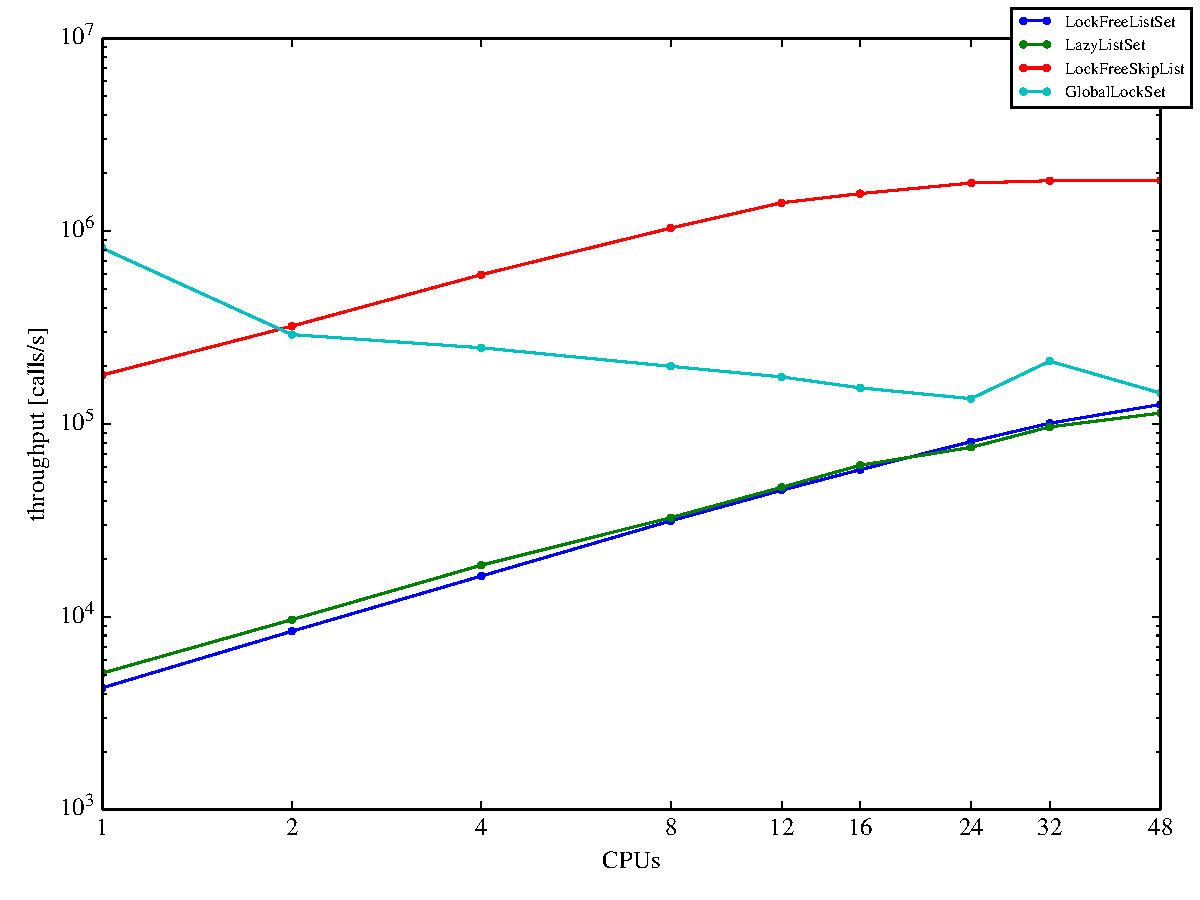
\includegraphics[width=0.9\linewidth]{figures/add}
  \caption{Comparison of node-insertion throughput for various thread-safe set implementations.}
  \label{add}
\end{figure}


\begin{figure}[htb]
  \centering
  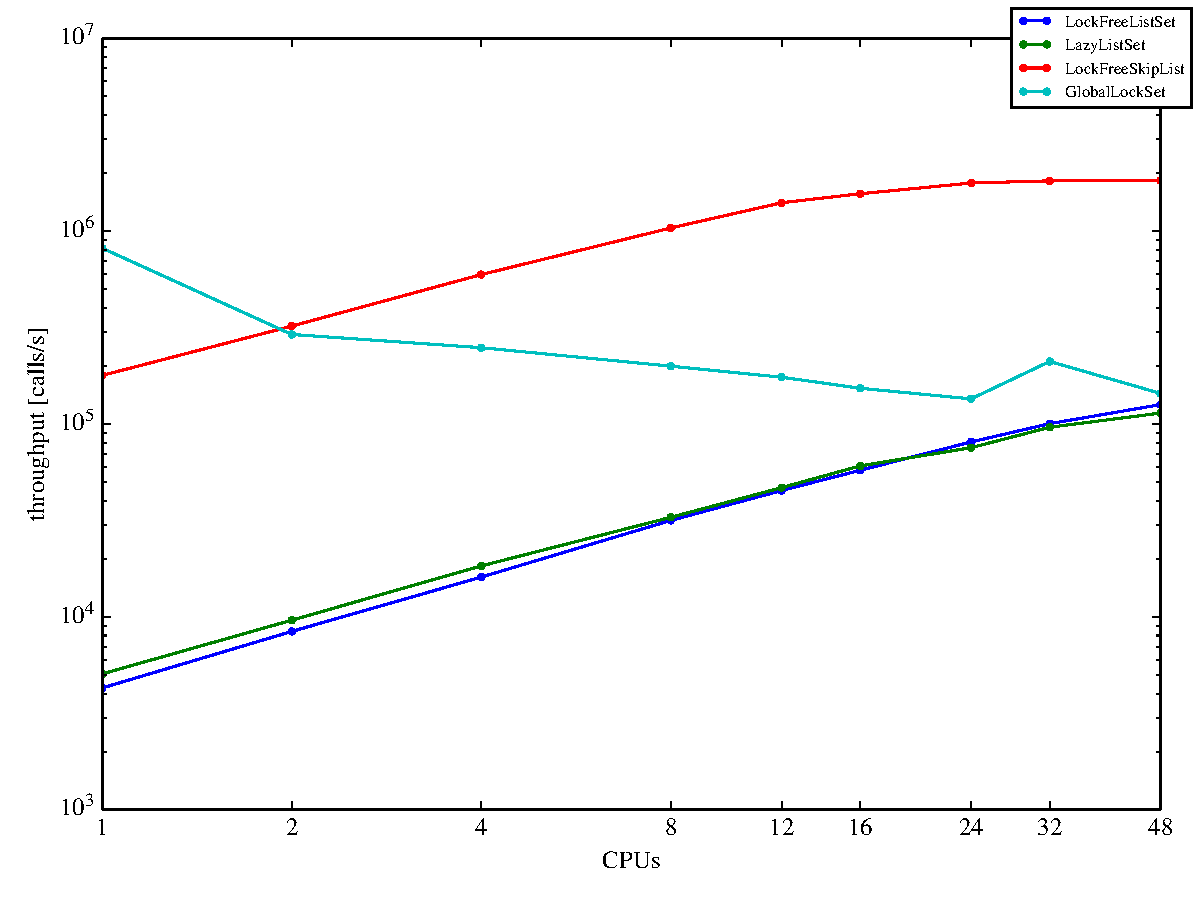
\includegraphics[width=0.9\linewidth]{figures/remove}
  \caption{Comparison of node-removal throughput for various thread-safe set implementations.}
  \label{remove}
\end{figure}


\begin{figure}[htb]
  \centering
  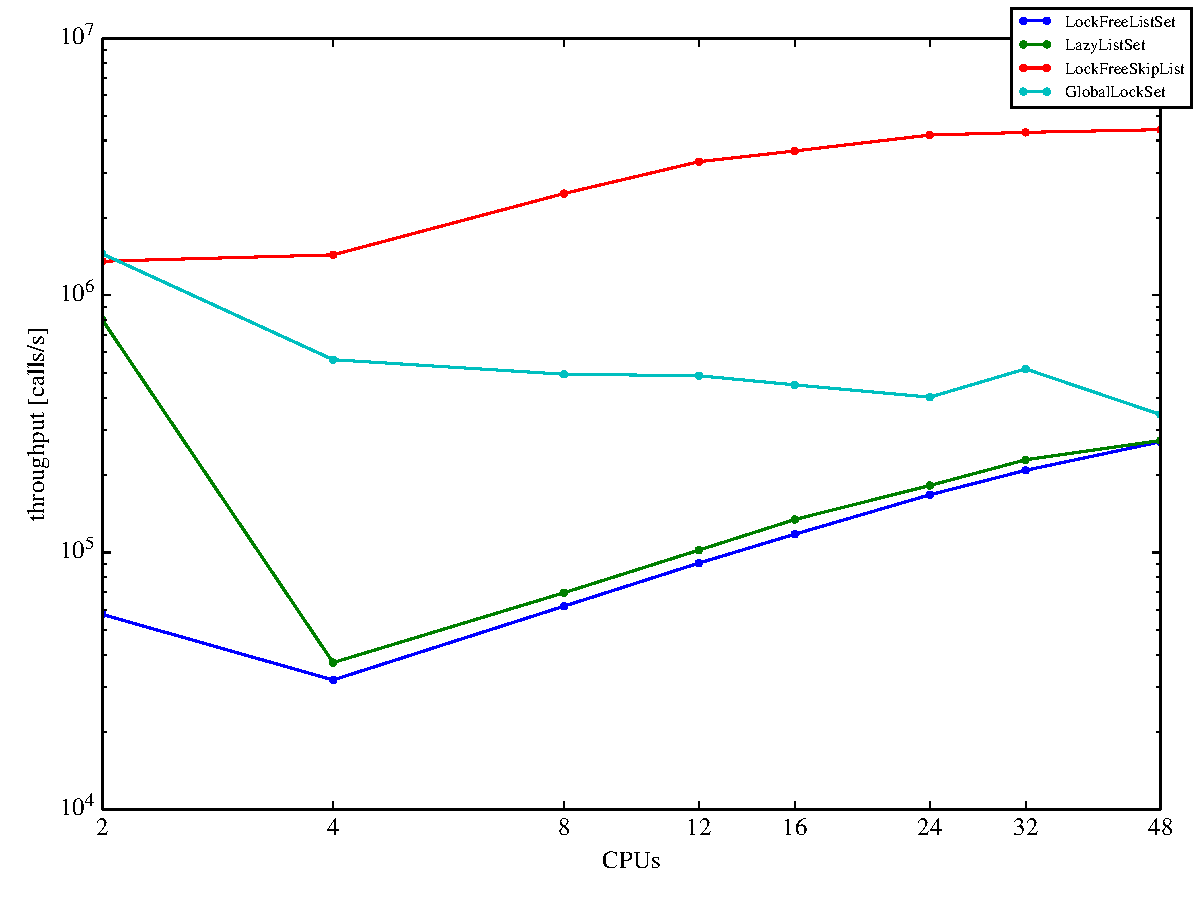
\includegraphics[width=0.9\linewidth]{figures/contains}
  \caption{Comparison of set query throughput for various thread-safe set implementations.}
  \label{contains}
\end{figure}


The throughput plots for node insertion and removal look very similar.
In both cases the highly optimized \texttt{std::set} outperforms all other data-structures in single-threaded use-cases.
However its performance quickly deteriorates with more threads due to the global locking while the other lock-free or fine-grain locked data structures improve throughput with more threads.
With 2 threads \texttt{LockFreeSkipList} already starts to outperform \texttt{GlobalLockSet}.
With 48 threads the list-based sets almost reach its throughput while \texttt{LockFreeSkipList} far exceeds it.

Figure \ref{contains} shows the throughput for set queries and mostly mirrors the results for node insertion and removal.
The only difference being that list-based sets perform significantly better for 2 threads than for more than two.
One explanation for this could in the way nodes get added and removed for stress testing with 2 threads creating an ideal producer-consumer relation for sorted list based sets.

As can be seen the lock-free skip list outperforms all other tested data-structures in all cases safe for the single-threaded one.

\end{document}